\documentclass{standalone}
\PassOptionsToPackage{dvipsnames}{xcolor}
\usepackage{tikz}
\usetikzlibrary{decorations,positioning,fadings,through,arrows.meta,shadows}
\usepackage{pgfplotstable}
\usepackage{etoolbox}
\usepackage{bm}


\newcommand{\Plus}{%
\mathord{%
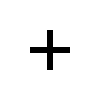
\begin{tikzpicture}[baseline=0ex, line width=2, scale=0.25]
\draw (1,0) -- (1,2);
\draw (0,1) -- (2,1);
\end{tikzpicture}}}

\newcommand{\Minus}{%
\mathord{%
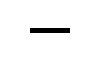
\begin{tikzpicture}[baseline=1ex, line width=2, scale=0.25]
\draw (0,1) -- (2,1);
\end{tikzpicture}}}

% https://tex.stackexchange.com/questions/14283/stroke-with-variable-thickness
\makeatletter
\pgfkeys{/pgf/decoration/.cd,
	start color/.store in =\startcolor,
	end color/.store in   =\endcolor,
	start width/.store in =\startwidth,
	end width/.store in   =\endwidth
}

\pgfdeclaredecoration{width and color change}{initial}{
	\state{initial}[width=0pt, next state=line, persistent precomputation={%
		\pgfmathdivide{50}{\pgfdecoratedpathlength}%
		\let\increment=\pgfmathresult%
		\def\x{0}%
	}]{}
	\state{line}[width=0.5pt,
	persistent postcomputation={%
		\pgfmathadd@{\x}{\increment}%
		\let\x=\pgfmathresult%
	}]{%
		\pgfsetlinewidth{\endwidth*(\x/100)+\startwidth*(100-\x)/100}%
		%\pgfsetlinewidth{\pgflinewidth}%
		\pgfsetarrows{-}%
		\pgfpathmoveto{\pgfpointorigin}%
		\pgfpathlineto{\pgfqpoint{0.75pt}{0pt}}%
		\pgfsetstrokecolor{\endcolor!\x!\startcolor}%
		\pgfusepath{stroke}%
	}
	\state{final}{%
		\pgfsetlinewidth{\endwidth}%
		\pgfpathmoveto{\pgfpointorigin}%
		%\pgfpathlineto{\pgfpointdecoratedpathlast\advance\pgf@... by2.0\pgflinewidth}%
		\color{\endcolor!\x!\startcolor}%
		\pgfusepath{stroke}% 
	}
}
\makeatother

% Parameters
\newcommand\timetext[1]{\LARGE#1}

%\def\inputname{FlatInitLinearRight}
%\def\inputname{HeFlatRight}
%\def\inputname{FlatInitRight}
\def\inputname{ComplexFlatBig}

%\def\inputname{ComplexDeepBig}
%\def\inputname{HeDeepLeft}
%\def\inputname{HeDeepMiddle}
%\def\inputname{HeDeepRight}

\def\xstretch{15}
\def\xstretchcm{\xstretch cm}
\def\ystretch{5.5}
\def\minnodesize{5}
\def\nodemul{5}
\def\nodeopacity{0.6}
\def\minwidth{0.5}
\def\widthmulti{1}
\def\edgeopacity{0.3}
\colorlet{locol}{darkgray!30!white}
\colorlet{hicol}{RoyalPurple}


\definecolor{col7}{HTML}{0495f5}
\definecolor{col8}{HTML}{ed5300}

\definecolor{col0}{HTML}{5506ff}
\definecolor{col1}{HTML}{e3009f}
\definecolor{col2}{HTML}{ffbb00}
\definecolor{col3}{HTML}{90c901}

% Axis-function colors
\colorlet{lightgray}{gray!10!white}
\definecolor{fline}{HTML}{6d87a1}
\colorlet{fbg}{white!15!lightgray}

\newcommand\col[1]{col#1}

\pgfplotstableread{data/\inputname/nodes.txt}\ntable
\pgfplotstablegetrowsof{\ntable}
\pgfmathsetmacro{\nrows}{\pgfplotsretval-1}
\pgfplotstableread{data/\inputname/times.txt}\ttable
\pgfplotstablegetrowsof{\ttable}
\pgfmathsetmacro{\trows}{\pgfplotsretval-1}
\pgfplotstableread{data/\inputname/options.txt}\opttable

\newtoggle{plotedges}
\toggletrue{plotedges}
\iftoggle{plotedges}{%
\pgfplotstableread{data/\inputname/edges.txt}\etable
\pgfplotstablegetrowsof{\etable}
\pgfmathsetmacro{\erows}{\pgfplotsretval-1}
}


\begin{document}
\begin{tikzpicture}[
  scale=1,
  nodestyle/.style={circle,draw=none,line width=0.3pt,minimum size=0pt,inner sep=0, anchor=center,opacity=\nodeopacity},
  edgestyle/.style={opacity=\edgeopacity},
  axisstyle/.style={|-|,darkgray!50!white,line width=1.6pt},
  ashadow/.style={opacity=0.25,shadow xshift=0.08,shadow yshift=-0.1},
  nodeshadow/.style={drop shadow={ashadow, color=white!60!black}},
  lineshadow/.style={preaction={transform canvas={shift={(0.06,-0.08)}},draw=white!60!black,thick,opacity=0.25}}
  ]
  
  \pgfplotstablegetelem{0}{[index]0}\of\opttable
  \xdef\xmin{\pgfplotsretval}
  \pgfplotstablegetelem{0}{[index]1}\of\opttable
  \xdef\xmax{\pgfplotsretval}
  \pgfplotstablegetelem{0}{[index]2}\of\opttable
  \xdef\xlo{\pgfplotsretval}
  \pgfplotstablegetelem{0}{[index]3}\of\opttable
  \xdef\xhi{\pgfplotsretval}
  \pgfplotstablegetelem{0}{[index]4}\of\opttable
  \xdef\ylo{\pgfplotsretval}
  \pgfplotstablegetelem{0}{[index]5}\of\opttable
  \xdef\yhi{\pgfplotsretval}
  
  \colorlet{epochfill}{white}
  
  % epoch text node
  \node[draw=darkgray!70!white,fill=epochfill,line width=1pt,anchor=north,inner sep=8pt] (bar) at (-0.7, \ystretch-0.7) {\LARGE Epochs};
  \node[draw=none,inner sep=8pt,anchor=north] (foo) at (-1.2, \ystretch-0.7) {};
  
  % axes and epoch number nodes
  \foreach \row in {0,...,\trows} {
	\node[minimum size=0,inner sep=0] (s\row) at (-0*\xstretchcm, -\ystretch*\row) {};
	\node[minimum size=0,inner sep=0] (e\row) at (1*\xstretchcm, -\ystretch*\row) {};
	\draw[axisstyle] (s\row) -- (e\row);
	\pgfplotstablegetelem{\row}{[index]0}\of\ttable
	\xdef\time{\pgfplotsretval}
	\node[circle,draw=darkgray!70!white,fill=epochfill,line width=1pt,anchor=center,minimum size=40pt] (foo\row) at (-1.2, 2.15-\ystretch*\row) {\timetext{\time}};
  }

  % xmin xmax
  \node[anchor=south] (a0) at (0, -1.0-\ystretch*0) {\LARGE$\xmin$};
  \node[anchor=south] (b0) at (\xstretchcm, -1.0-\ystretch*0) {\LARGE$\xmax$};
  \pgfmathsetmacro\zat{\xstretch*(-\xmin/(\xmax-\xmin)}
  \node[anchor=south] (z0) at (\zat cm, -1.0-\ystretch*0) {\LARGE$0$};

  % epoch lines
  \def\tipwl{8pt}
  \def\heightpm{1.6cm}
  \node[draw=none, below=\heightpm of foo0] (afterfoo0) {};
  \draw[-,darkgray!70!white,line width=1pt] (foo) -- (foo0.north);
  \draw[-{Turned Square[open,length=\tipwl,width=\tipwl]},darkgray!70!white,line width=1pt] (foo0) -- (afterfoo0.north);
  \foreach \row in {1,...,\trows} {
    \pgfmathsetmacro\prevrow{int(\row-1)}
  	\node[draw=none, above=\heightpm of foo\row] (beforefoo\row) {};
  	\node[draw=none, below=\heightpm of foo\row] (afterfoo\row) {};
  	\draw[{Turned Square[open,length=\tipwl,width=\tipwl]}-,darkgray!70!white,line width=1pt] (beforefoo\row) -- (foo\row.north);
  	\draw[-{Turned Square[open,length=\tipwl,width=\tipwl]},darkgray!70!white,line width=1pt] (foo\row) -- (afterfoo\row.north);
  }

  % draw epoch nodes again to cover line shadows
  \foreach \row in {0,...,\trows} {
	\pgfplotstablegetelem{\row}{[index]0}\of\ttable
	\xdef\time{\pgfplotsretval}
	\node[circle,draw=darkgray!70!white,fill=epochfill,line width=1pt,anchor=center,minimum size=40pt] (foo\row) at (-1.2, 2.15-\ystretch*\row) {\timetext{\time}};
  }

  \foreach \row in {0,...,\nrows} {
	\pgfplotstablegetelem{\row}{[index]0}\of\ntable
	\xdef\noderow{\pgfplotsretval}
	\pgfplotstablegetelem{\row}{[index]1}\of\ntable
	\xdef\nodecol{\pgfplotsretval}
	\pgfplotstablegetelem{\row}{[index]2}\of\ntable
	\xdef\nodepos{\pgfplotsretval}
	\pgfplotstablegetelem{\row}{[index]3}\of\ntable
	\xdef\nodecolor{\pgfplotsretval}
	\colorlet{nodecol}{\col{\nodecolor}}
	%\colorlet{nodecol}{hicol!\nodecolor!locol}
	\pgfplotstablegetelem{\row}{[index]4}\of\ntable
	\xdef\nodesize{\minnodesize+\nodemul*\pgfplotsretval}
	\node [nodestyle,fill=nodecol,minimum size=\nodesize] (\noderow/\nodecol) at (\xstretchcm*\nodepos, -\ystretch*\noderow) {};
  }

  \iftoggle{plotedges}{%
  \foreach \row in {0,...,\erows} {
	\pgfplotstablegetelem{\row}{[index]0}\of\etable
	\xdef\srow{\pgfplotsretval}
	\pgfplotstablegetelem{\row}{[index]1}\of\etable
	\xdef\scol{\pgfplotsretval}
	\pgfplotstablegetelem{\row}{[index]2}\of\etable
	\xdef\trow{\pgfplotsretval}
	\pgfplotstablegetelem{\row}{[index]3}\of\etable
	\xdef\tcol{\pgfplotsretval}
	% Colors
	\pgfplotstablegetelem{\row}{[index]4}\of\etable
	\xdef\sclr{\pgfplotsretval}
	\colorlet{cstart}{\col{\sclr}}
	\pgfplotstablegetelem{\row}{[index]5}\of\etable
	\xdef\tclr{\pgfplotsretval}
	\colorlet{cend}{\col{\tclr}}
	%\colorlet{cend}{hicol!\tclr!locol}
	% Widths
	\pgfplotstablegetelem{\row}{[index]6}\of\etable
	\xdef\swidth{\minwidth + \widthmulti*\pgfplotsretval}
	\pgfplotstablegetelem{\row}{[index]7}\of\etable
	\xdef\twidth{\minwidth + \widthmulti*\pgfplotsretval}
	%\draw [decoration={width and color change, start color=darkgray!80!white, end color=darkgray!80!white, start width=1.5*\swidth, end width=1.5*\twidth}, decorate] (\srow/\scol.center) to [out=-90,in=90,looseness=0.8] (\trow/\tcol.center);
	%\draw [edgestyle, color=cstart, line width=1.5*\twidth] (\srow/\scol) to [out=-90,in=90,looseness=0.4] (\trow/\tcol);
	\draw [edgestyle, smooth, color=cstart, line width=1.5*\twidth] (\srow/\scol) -- (\trow/\tcol);
	%\draw [decoration={width and color change, start color=cstart, end color=cend, start width=\swidth, end width=\twidth}, decorate] (\srow/\scol.center) to [out=-90,in=90,looseness=0.8] (\trow/\tcol.center);
  }
  }

  \foreach \row in {0,...,\trows} {
  \pgfmathsetmacro\xat{(\xlo-\xmin)*\xstretch/(\xmax-\xmin)}
  \pgfmathsetmacro\xwidth{(\xhi-\xlo)*\xstretch/(\xmax-\xmin)}
  \begin{axis}[%
    anchor=south west,
    at={(\xat*1cm,-\row*\ystretch cm + 0.5cm)},
    axis y line=none,
    axis line style={
    	darkgray!80!white,
    	line width=1pt
    },
    axis background/.style={fill=fbg, opacity=0.8},
    width=\xwidth*1cm,
    height=3.8cm,
    xmin=\xlo,
    xmax=\xhi,
    ymin=\ylo,
    ymax=\yhi,
    ticks=none,
    restrict y to domain=-100:100,
    clip mode=individual,
    clip=true,
    scale only axis
  ]

  %\node[draw=black,fill=white!80!lightgray,minimum height=0.9cm,text width=2.4cm,anchor=south west] (zoom\row) at (axis cs: -0.15,-9.5) {};
  %\node[draw=none,above=2cm of zoom\row] (bzoom\row) {};
  %\draw[black] (zoom\row) -- (bzoom\row);
  
  \addplot[%
    only marks,
    mark=square*,
    mark size=5pt,
    mark options={darkgray}
  ] table[col sep=comma] {data/\inputname/data.txt};

  \addplot[%
    mark=none,
    fline!10!white,
    line width=4pt
  ] table[col sep=comma] {data/\inputname/xy_\row.txt};

  \addplot[%
    mark=none,
    fline,
    line width=3pt
  ] table[col sep=comma] {data/\inputname/xy_\row.txt};
  
  %\node[draw=black,fill=none,minimum height=0.9cm,text width=2.4cm,anchor=south west] (czoom\row) at (axis cs: -0.15,-9.5) {};

  \end{axis}
  }

  \xdef\xmin{-0.2}
  \xdef\xmax{2.2}
  \xdef\xlo{-0.2}
  \xdef\xhi{2.2}
  \xdef\ylo{-1.5}
  \xdef\yhi{2}
  
%  \foreach \row in {0,...,\trows} {
%	\pgfmathsetmacro\xat{(\xlo-\xmin)*10/(\xmax-\xmin)}
%	\pgfmathsetmacro\xwidth{(\xhi-\xlo)*10/(\xmax-\xmin)}
%  	
%	\begin{axis}[%
%	anchor=south west,
%	at={(\xat*1cm + 6.2cm,-\row*\ystretch cm + 3.2cm)},
%	%axis y line=none,
%	axis line style={
%		black,
%		line width=0.6pt
%	},
%	axis background/.style={
%		fill=white!80!lightgray,
%		opacity=1.0,
%	},
%	width=\xwidth*1cm,
%	height=3.2cm,
%	xmin=\xlo,
%	xmax=\xhi,
%	ymin=\ylo,
%	ymax=\yhi,
%	ticks=none,
%	restrict y to domain=-100:100,
%	clip mode=individual,
%	clip=true,
%	scale only axis,
%	axis on top
%	]
%  	
%	\addplot[%
%	only marks,
%	mark=square*,
%	mark size=5pt,
%	mark options={darkgray}
%	] table[col sep=comma] {data/\inputname/data.txt};
%	
%	\addplot[%
%	mark=none,
%	darkgray!40!Goldenrod,
%	line width=3pt
%	] table[col sep=comma] {data/\inputname/xy_\row.txt};
%	
%	\end{axis}
%	
%  }

  \iftoggle{plotedges}{%
  	%\node[draw=none] (corner) at (current bounding box.north east) {};
  	%\node[draw=none,above=0.2cm of corner] (pushcorner) {};
    \node[draw=darkgray!70!white,fill=white,minimum width=2.25cm,minimum height=2.4cm,line width=1pt,anchor=north east,nodeshadow] at (current bounding box.north east) {};

    \node[draw=none,anchor=north east,inner sep=10pt,text width=1.15cm] at (current bounding box.north east) {\Huge $a_i$};

    \node[circle,draw=none,anchor=north east,inner sep=4pt] (legref) at (current bounding box.north east) {};

    \def\colnodems{0.85cm}
    \def\colnodexoff{0.06}
    \pgfmathsetmacro\colnodexl{0.95+\colnodexoff}
    \pgfmathsetmacro\colnodexr{0.0+\colnodexoff}
    \def\colnodeyoff{1}
    \pgfmathsetmacro\colnodeyt{0.0+\colnodeyoff}
    \pgfmathsetmacro\colnodeyb{0.95+\colnodeyoff}

    \node[circle,draw=none,fill=col8,anchor=north east,inner sep=0,minimum size=\colnodems,below left = \colnodeyt cm and \colnodexl cm of legref] {\color{white}\LARGE $\Plus$};
    \node[circle,draw=none,fill=col7,anchor=north east,inner sep=0,minimum size=\colnodems,below left = \colnodeyt cm and \colnodexr cm of legref] {\color{white}\LARGE $\Minus$};
  }{%
  	%\node[draw=none] (corner) at (current bounding box.north east) {};
    %\node[draw=none,above=0.2cm of corner] (pushcorner) {};
    \node[draw=darkgray!70!white,fill=white,minimum width=2.25cm,minimum height=3.1cm,line width=1pt,anchor=north east,nodeshadow] at (current bounding box.north east) {};
  
    \node[draw=none,anchor=north east,inner sep=8pt,text width=1.65cm] at (current bounding box.north east) {\LARGE Layers};
  
    \node[circle,draw=none,anchor=north east,inner sep=4pt] (legref) at (current bounding box.north east) {};
  
    \def\colnodeis{3pt}
    \def\colnodexoff{0.06}
    \pgfmathsetmacro\colnodexl{0.95+\colnodexoff}
    \pgfmathsetmacro\colnodexr{0.0+\colnodexoff}
    \def\colnodeyoff{0.9}
    \pgfmathsetmacro\colnodeyt{0.0+\colnodeyoff}
    \pgfmathsetmacro\colnodeyb{0.95+\colnodeyoff}
  
    \node[circle,draw=none,fill=col0,anchor=north east,inner sep=\colnodeis,below left = \colnodeyt cm and \colnodexl cm of legref] {\color{white}\LARGE \textbf{1}};
    \node[circle,draw=none,fill=col1,anchor=north east,inner sep=\colnodeis,below left = \colnodeyt cm and \colnodexr cm of legref] {\color{white}\LARGE \textbf{2}};
    \node[circle,draw=none,fill=col2,anchor=north east,inner sep=\colnodeis,below left = \colnodeyb cm and \colnodexl cm of legref] {\color{white}\LARGE \textbf{3}};
    \node[circle,draw=none,fill=col3,anchor=north east,inner sep=\colnodeis,below left = \colnodeyb cm and \colnodexr cm of legref] {\color{white}\LARGE \textbf{4}};
  }

  \node[draw=darkgray!70!white,fill=epochfill,line width=1pt,anchor=north,inner sep=8pt,nodeshadow] (bar) at (-0.7, \ystretch-0.7) {\LARGE Epochs};


\end{tikzpicture}
\end{document}